\subsection{Hubble Constant from $\chi$ Dynamics}
  \label{subsec:hubble-constant-from-chi-dynamics}

  In Cosmochrony, the Hubble parameter is not introduced as a free cosmological
  constant, but arises as an effective quantity associated with the relaxation
  dynamics of the $\chi$ substrate.
  At the level of an effective spacetime description, it may be written as
  \begin{equation}
    H(t) = \frac{\dot{\chi}}{\chi},
  \end{equation}
  where the dot denotes differentiation with respect to an effective cosmological
  time parameter introduced solely to parametrize the relaxation ordering, not a
  fundamental temporal evolution.

  In homogeneous regimes, the relaxation rate approaches its maximal admissible
  value.
  Assuming $\dot{\chi}_{\mathrm{eff}} \simeq c$, the present-day Hubble parameter can
  be estimated as
  \begin{equation}
    H_0 \simeq \frac{c}{\chi(t_0)}.
  \end{equation}

  This relation establishes a direct correspondence between the observed Hubble
  constant and the characteristic relaxation scale of $\chi$ at the current epoch.
  Early-universe probes (such as CMB-based inferences) and late-time distance-ladder
  measurements effectively sample $\chi$ at different stages of its relaxation,
  naturally leading to systematically different inferred values of $H_0$ without
  invoking additional cosmological components or fine-tuned initial conditions.

% Requires: \usepackage{pgfplots}
% Optional: \pgfplotsset{compat=1.18}
  \begin{figure}[t]
    \centering
    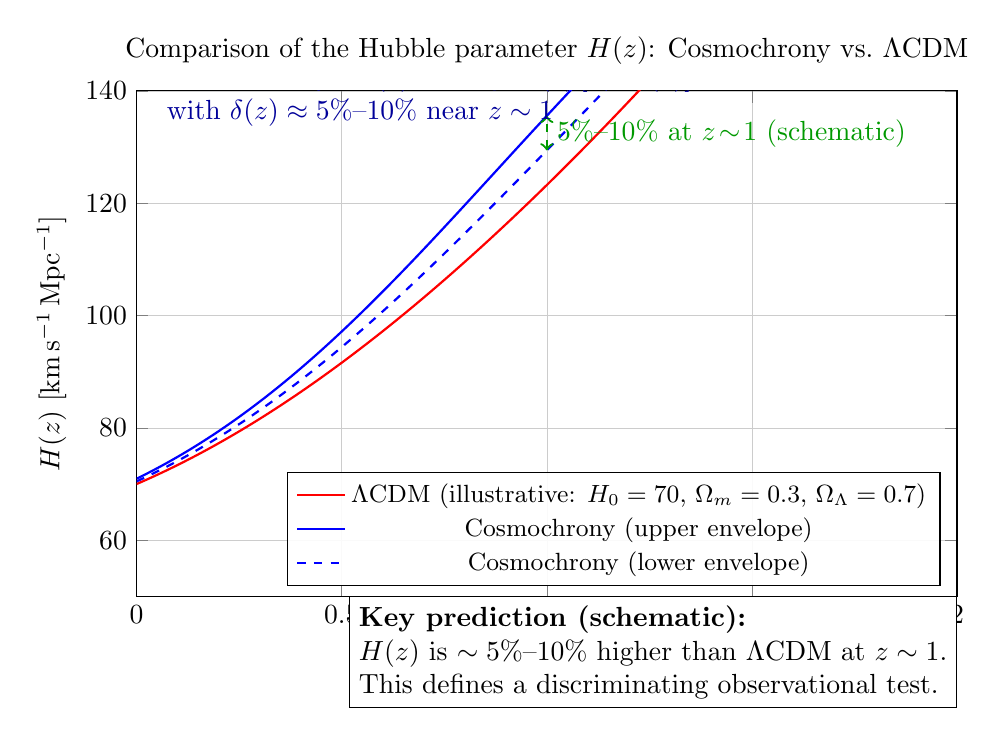
\begin{tikzpicture}
      \begin{axis}[
        width=12cm,
        height=8cm,
        title={Comparison of the Hubble parameter $H(z)$: Cosmochrony vs.\ $\Lambda$CDM},
      xlabel={Redshift $z$},
      ylabel={$H(z)$ [km\,s$^{-1}$\,Mpc$^{-1}$]},
      xmin=0, xmax=2,
      ymin=50, ymax=140,
      xtick={0,0.5,1,1.5,2},
      legend style={
        at={(rel axis cs:0.98,0.02)},
        anchor=south east,
        draw=black,
        fill=white,
        fill opacity=0.9,
        text opacity=1,
        font=\small
      },
      grid=both,
      grid style={line width=.1pt, draw=gray!10},
      major grid style={line width=.2pt, draw=gray!40},
      ]

        % --- Baseline LCDM (flat, matter+Lambda; schematic but standard form) ---
        % Choose H0=70, Om=0.3, Ol=0.7 as illustrative values.
        \addplot[
          domain=0:2, samples=200,
          red, thick, mark=none
        ]
        {70*sqrt(0.3*(1+x)^3 + 0.7)};
        \addlegendentry{$\Lambda$CDM (illustrative: $H_0=70$, $\Omega_m=0.3$, $\Omega_\Lambda=0.7$)}

        % --- Cosmochrony: prediction band (5-10% higher around z~1) ---
        % Use a smooth bump centered at z=1 to represent partial-projectability correction.
        % Band = LCDM * (1 + delta(z)), with delta in [5%,10%] near z~1.
        \addplot[
          domain=0:2, samples=200,
          blue, thick, mark=none
        ]
        {70*sqrt(0.3*(1+x)^3 + 0.7) * (1 + 0.10*exp(-2*(x-1)^2))};
        \addlegendentry{Cosmochrony (upper envelope)}

        \addplot[
          domain=0:2, samples=200,
          blue, thick, dashed, mark=none
        ]
        {70*sqrt(0.3*(1+x)^3 + 0.7) * (1 + 0.05*exp(-2*(x-1)^2))};
        \addlegendentry{Cosmochrony (lower envelope)}

        % Highlight at z=1 (automatic from functions would be nicer; fixed coords acceptable if consistent)
        \draw[<->, thick, dashed, green!60!black]
        (axis cs:1, {70*sqrt(0.3*(2)^3 + 0.7) * (1 + 0.05*exp(-2*(0)^2))})
        --
        node[right, green!60!black] {$5\%$--$10\%$ at $z\!\sim\!1$ (schematic)}
        (axis cs:1, {70*sqrt(0.3*(2)^3 + 0.7) * (1 + 0.10*exp(-2*(0)^2))});

        % Annotation
        \node[align=left, anchor=south west, blue!60!black]
        at (axis cs:0.05,132)
          {Cosmochrony: $H(z)=H_{\Lambda\mathrm{CDM}}(z)\,[1+\delta(z)]$\\
        with $\delta(z)\approx 5\%$--$10\%$ near $z\sim 1$};

      \end{axis}

      \node[draw, align=left, fill=white, anchor=north east]
      at (rel axis cs:1,0) {
        \textbf{Key prediction (schematic):}\\
        $H(z)$ is $\sim 5\%$--$10\%$ higher than $\Lambda$CDM at $z\sim 1$.\\
        This defines a discriminating observational test.
      };
    \end{tikzpicture}
    \caption{Schematic comparison of $H(z)$ in Cosmochrony and $\Lambda$CDM.
    The $\Lambda$CDM curve uses the standard matter+$\Lambda$ functional form with illustrative parameters,
      while Cosmochrony is represented as a fractional enhancement band near $z\sim 1$.}
    \label{fig:hubble-comparison}
  \end{figure}
